\chapter{Mathematical Formulation}
\label{mathchapter}

The objective of this fake thesis document is to demonstrate some
\LaTeX{} features as well as features specific to the thesis class.
We start by giving one short formula, 
\begin{equation}
	A = \pi r^2,
\end{equation}
and one big hairy multi-line
formula (one of the non-dimensional Navier-Stokes equations):
\begin{eqnarray}
  \rho \left[ \frac{DV_r}{Dt} - M \epsilon^2
    \frac{V_\theta^2}{r} \right]
  & = & -\frac{\delta^2}{\gamma~ M} \frac{\partial P}{\partial r}
	+ \frac{M ~\delta^2}{Re} \left\{ 2 \frac{\partial }{\partial r}
	\left[ \mu \left( \frac{\partial V_r}{\partial r}
        - \frac{1}{3} {\bf \nabla \cdot \overline{V}}
      \right) \right] \right. \nonumber \\
  & & + \frac{1}{r} \frac{\partial }{\partial \theta} \left[ \mu \left(
      \frac{1}{r} \frac{\partial V_r}{\partial \theta} + \epsilon \frac{\partial V_{\theta}}{\partial r}
      - \epsilon \frac{V_{\theta}}{r} \right) \right] \nonumber \\
  & & + \frac{\partial }{\partial z} \left[ \mu \left( \frac{1}{\delta^2}
        \frac{\partial V_r}{\partial z} + \frac{\partial V_z}{\partial r} \right) \right] \nonumber \\
  & & + 2 \left. \frac{\mu}{r}\left[ \frac{\partial V_r}{\partial r} -\frac{\epsilon}{r}
      \frac{\partial V_{\theta}}{\partial \theta} - \frac{V_r}r\right] \right\}, \label{eq:rmom}
\end{eqnarray}
The latter equation is non-dimensionalized using the following definitions:
\begin{displaymath}
	r = \frac{r'}{R'}, \quad
	z = \frac{z'}{L'}, \quad
	t = \frac{t'}{t_a'}, \quad
	\kappa = \frac{\kappa'}{\kappa_0'}, \quad
	\mu = \frac{\mu'}{\mu_0'} , \quad
	C_V = \frac{C_V'}{C_{V0}'},
      \end{displaymath}
where $P_0'$ is the initial static pressure in the cylinder,
and $\rho_0'$ and $T_0'$ are the density and temperature
of the fluid being injected from the sidewall.
The aspect ratio is given by $\delta = \frac{L'}{R'}$,
where $\delta \gg 1$.
The induced characteristic axial velocity and the characteristic
endwall velocity disturbance $V_{z0}'$ is defined with respect
to the injection reference sidewall velocity,
$V_{r0}'$ by overall mass conservation,
$\frac{V_{z0}'}{V_{r0}'} = \delta$.
The size of the initially unknown reference
azimuthal velocity $V_{\theta 0}'$ is related to
$V_{r0}'$ by $\frac{V_{\theta 0}'}{V_{r0}'}=\epsilon$.
Later, it is shown that $\epsilon=1$.

\begin{figure}
\centerline{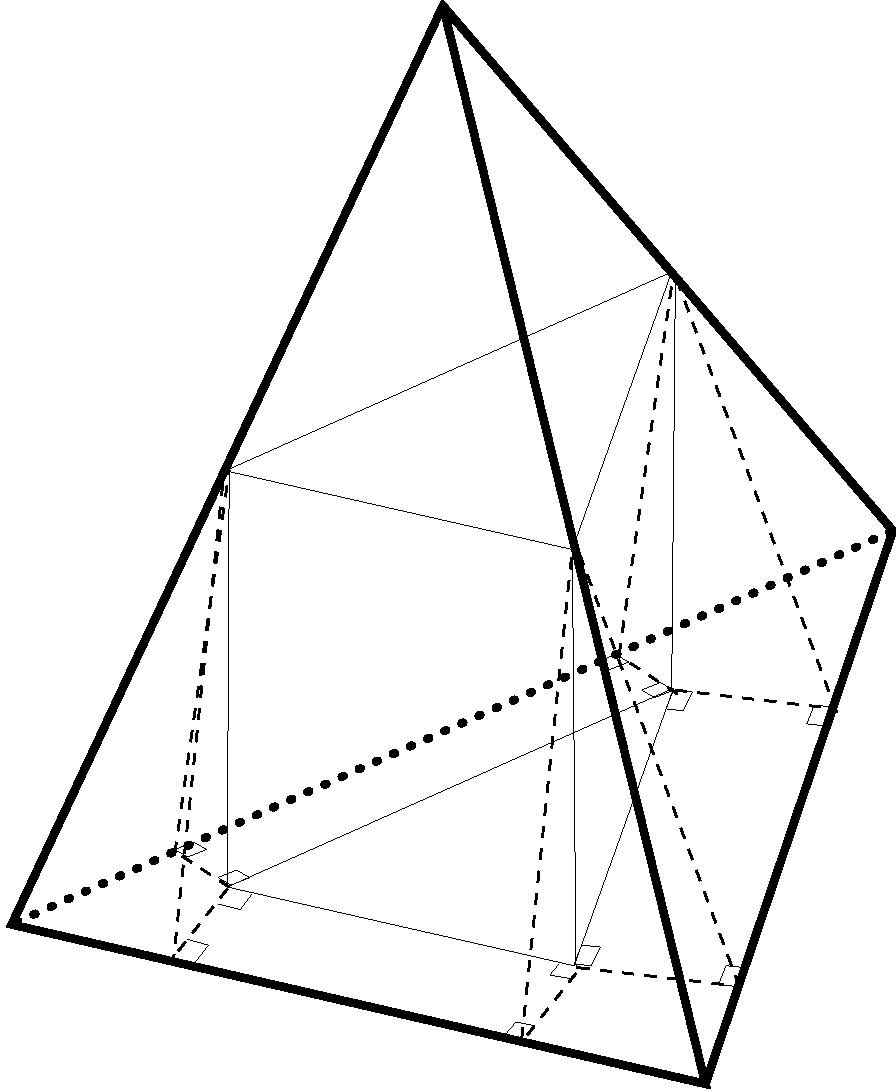
\includegraphics[height=95mm]{pyr}}
\caption[Cutting up a triangular pyramid]{
	A triangular pyramid may be cut up as shown, to
	yield one top pyramid (with one-eighth the volume
	of the full pyramid), three bottom corner pyramids
	(which, when joined, are congruent to the top pyramid),
	three prisms along the bottom edges (the area of whose
	bottom faces total $B/2$) and the large central prism
	(volume = $(B/4)(h/2) = Bh/8$).
	The image, from PostScript file ``pyr.eps'',
	was read in using the {\tt $\backslash$includegraphics}
	command, from the {\tt graphicx} package.
	}
\label{fig:pyramid}
\end{figure}

The time is non-dimensionalized using the
axial acoustic time scale,
$t_a'=\frac{L'}{C_0'}$, where
$C_0'=(\gamma {\cal R} ' T_0')^{\frac12}$
is the speed of
sound,\footnote{In air at 1 atm., $\frac{1 mi.}{5 s}$.}
$\cal{R}'$ is the gas constant,
and $\gamma$ is the ratio of specific heats.
Also the Reynolds number, Wrenchl number,
and Mock number are defined as
\begin{displaymath}
	Re = \frac{\rho' V_{z_0}' L'}{ \mu_0'}, \quad
	Wr = \frac{\mu_0' C_{p_0}'}{\kappa_0'}, \quad
	M = \twovec{V_{z_0}'}{C_0'} \cdot
		\twomatrix{8a}{z_0-\rho}2{z_0-\mu} \twovec{Wr}{p-7},
\end{displaymath}
where $Re\ll1$, $M\gg1$, and $Wr=O(1)$.

Here is an example of using the \texttt{singlespace} environment.

\begin{singlespace}
  This paragraph was surrounded by the \texttt{singlespace}
  environment. The Mock number is chosen as a small parameter to
  model the small magnitude found in a typical rocket motor chamber,
  as opposed to the rocket nozzle where larger values are
  possible.\footnote{Not just possible, desirable!} The aspect
  ratio, $\delta$, is taken to be a large parameter, because many
  chambers have aspect ratios between 15 and 50.
\end{singlespace}

The following table is created using the \LaTeX{}
\texttt{tabular} environment.

\begin{table}
\begin{center}
\label{tbl:sample2}
\caption[Yet another {\tt tabular} table]{
	This is a table constructed with \LaTeX{}
	commands in the {\tt tabular} environment.
	}
   \begin{tabular}{|c||c|c|c|c||c|} \hline
   n & $n^2$ & $n^3$ & $n^4$  & $n^7$ & $n^{13}$ \cr \hline \hline
   2 &  4  &  8  &   16    &    128  & 8192 \cr
   3 &  9  &  27  &   81    &   2187  & 1594323 \cr \hline
   4 &  16  &  64  &   256   &  16384  & 67108864 \cr
   5 &  25  &  125  &   625  &  78125  & 1220703125 \cr \hline
   6 &  36  &  216  &   1296 &  279936  & 13060694016 \cr
   7 &  49  &  343  &   2401 &  823543  & 96889010407 \cr \hline
   \end{tabular}
\end{center}
\end{table}

However, sometimes you want to use a table produced by some other
software, such as Excel.  If the table is saved to a PostScript file,
then it can be displayed using the $\backslash${\tt includegraphics}
macro inside a {\tt table} environment:

\begin{table}
  \caption[Table from a PostScript file]{\label{tbl:sample3}
   Table from a PostScript file. This table wasn't constructed with
   \LaTeX\ commands, but resides in a PostScript file
   ({\tt tableD.eps}) created by some other software.}
  \vspace{2ex}
  \centerline{\includegraphics[width=\textwidth]{tableD}}
\end{table}

\section{Conditions for Catastrophic Combustion}
\label{sec:cata}

Initially, a steady flow is generated by the sidewall injection,
$V_r = -V_{rws}(z)$. The subscript $srw$ is used to mean that there
is a {\bf s}teady {\bf r}adial {\bf w}all velocity. The sign is
negative due to the injection toward centerline. At $t=0^+$, the
endwall begins oscillating with the non-dimensionalized sinusoidal
axial velocity, $V_z=\widetilde{F}_{rw}(r,\theta,t)$, for $\omega =
O(1)$.

Some of the boundary conditions are:
\begin{eqnarray}
  z=0; && V_z = \twochoices
	{0, && t\leq0}
	{\widetilde{F}_{zw}(r,\theta,t), && t>0}
						\label{eq:endwall} \\
  z=0; && V_{\theta}=V_r=0,			\label{eq:endnoslip} \\
  r=0; && P,\rho,T,V_r,V_{\theta},V_z~\mbox{finite},	\label{eq:centerline} \\
  r=1; && V_r= F_{rws}(z),			\label{eq:injection} \\
  r=1; && V_z=V_{\theta} =0,				\label{eq:sidenoslip}
\end{eqnarray}
and solutions must be periodic in $\theta$.


\section{More Boundary Conditions}
\label{sec:bcs}

Initially, a steady flow is generated by the
sidewall injection, $V_r = -V_{rws}(z)$.
The sign is negative due to the injection toward
centerline.\footnote{This convention was
suggested by Goddard and Smythe.}
At $t=0^+$, the endwall begins oscillating with the
non-dimensionalized sinusoidal axial velocity,
$V_z =\widetilde{F}_{rw}(r,\theta,t)$,
for $\omega = O(1)$.
The frequency condition chosen represents the
first few axial acoustic modes observed in high
aspect ratio chambers.\footnote{Toy rockets,
the kind you used to shoot off with your dad
in the park, typically have only two significant
modes.}

The full boundary conditions include:
\begin{eqnarray}
  z=0; && V_{\theta}=V_r = 0,            \label{eqB:endnoslip} \\
  r=1; && V_r= \left\{
    \begin{array}{ll}
      F_{rws}(z), & t<0, \\
      F_{rws}(z)+\widetilde{F}_{rw}(z,\theta,t), & t\geq 0
    \end{array}
  \right.                               \label{eqB:injection} \\
  r=1; && V_z=V_{\theta} =0,                  \label{eqB:sidenoslip}
\end{eqnarray}
and solutions must be periodic in $\theta$.

If you don't believe this stuff, check out
Mulick \cite{mulick} and Baylor \cite{baylor}.

\subsection{Just Meaningless Text to Test Lines per Page
	\label{ss}}

Just meaningless text to test lines per page.
Just meaningless text to test lines per page.
Just meaningless text to test lines per page.
Just meaningless text to test lines per page.
Just meaningless text to test lines per page.
Just meaningless text to test lines per page.
Just meaningless text to test lines per page.
Just meaningless text to test lines per page.
Just meaningless text to test lines per page.
Just meaningless text to test lines per page.
Just meaningless text to test lines per page.
Just meaningless text to test lines per page.
Just meaningless text to test lines per page.
Just meaningless text to test lines per page.
Just meaningless text to test lines per page.
Just meaningless text to test lines per page.
Just meaningless text to test lines per page.
Just meaningless text to test lines per page.
Just meaningless text to test lines per page.
Just meaningless text to test lines per page.
Just meaningless text to test lines per page.
Just meaningless text to test lines per page.
Just meaningless text to test lines per page.
Just meaningless text to test lines per page.
Just meaningless text to test lines per page.
Just meaningless text to test lines per page.
Just meaningless text to test lines per page.
Just meaningless text to test lines per page.
Just meaningless text to test lines per page.
Just meaningless text to test lines per page.
Just meaningless text to test lines per page.
Just meaningless text to test lines per page.
Just meaningless text to test lines per page.
Just meaningless text to test lines per page.
Just meaningless text to test lines per page.
Just meaningless text to test lines per page.
Just meaningless text to test lines per page.
Just meaningless text to test lines per page.
Just meaningless text to test lines per page.
Just meaningless text to test lines per page.
Just meaningless text to test lines per page.
Just meaningless text to test lines per page.
Just meaningless text to test lines per page.
Just meaningless text to test lines per page.
Just meaningless text to test lines per page.
Just meaningless text to test lines per page.
Just meaningless text to test lines per page.
Just meaningless text to test lines per page.
Just meaningless text to test lines per page.
Just meaningless text to test lines per page.
Just meaningless text to test lines per page.
Just meaningless text to test lines per page.
Just meaningless text to test lines per page.
Just meaningless text to test lines per page.
Just meaningless text to test lines per page.
Just meaningless text to test lines per page.
Just meaningless text to test lines per page.
Just meaningless text to test lines per page.
Just meaningless text to test lines per page.
Just meaningless text to test lines per page.
Just meaningless text to test lines per page.
Just meaningless text to test lines per page.
Just meaningless text to test lines per page.
Just meaningless text to test lines per page.
Just meaningless text to test lines per page.
Just meaningless text to test lines per page.
Just meaningless text to test lines per page.
Just meaningless text to test lines per page.
Just meaningless text to test lines per page.
Just meaningless text to test lines per page.
Just meaningless text to test lines per page.
Just meaningless text to test lines per page.
Just meaningless text to test lines per page.
Just meaningless text to test lines per page.
Just meaningless text to test lines per page.
Just meaningless text to test lines per page.
Just meaningless text to test lines per page.
Just meaningless text to test lines per page.
Just meaningless text to test lines per page.
Just meaningless text to test lines per page.
Just meaningless text to test lines per page.
Just meaningless text to test lines per page.
Just meaningless text to test lines per page.
Just meaningless text to test lines per page.

\subsection{This Is a Subsection}

This is a subsection.
Filler filler filler filler filler filler filler filler.
Filler filler filler filler filler filler filler filler.

\subsection{This Is Another Subsection}

This is another subsection.
Filler filler filler filler filler filler filler filler.
Filler filler filler filler filler filler filler filler.

\paragraph{This Is a Paragraph}
It used a \verb2\paragraph{}2 header, which
are always inlined (with extra space)
and  boldfaced.

Filler filler filler filler filler filler filler filler.
Filler filler filler filler filler filler filler filler.

\paragraph{What Is It?}
This is a paragraph.
The heading of the paragraph is emphasized.
This is a paragraph.
The heading of the paragraph is emphasized.

\section{Sideways Tables}

In Table~\ref{tbl:sidewaysT} on page~\pageref{tbl:sidewaysT} we show
on a separate page how \LaTeX\ can handle big tables that need to be
put sideways. All we need to do is to put the table into a
\texttt{sidewaystable} environment. The rest is handled by \LaTeX.
In particular, we can easily make sure that the table will take just
the available space. That's neat, isn't it? Just make sure you load
the \texttt{rotating} package that defines the
\texttt{sidewaystable} environment.

\begin{sidewaystable}[ht]
  \caption{\label{tbl:sidewaysT}A big table that needs to go
   sideways -- easy with \LaTeX.}

  \vspace{2ex}
  \renewcommand{\arraystretch}{1.2}
  \begin{tabular*}{\textwidth}{@{\extracolsep{\fill}}*{26}{r}}
    \hline\hline
    a & b & c & d & e & f & g & h & i & j & k & l & m & n & o &
     p & q & r & s & t & u & v & w & x & y & z
    \\ \hline
    1 & 2 & 3 & 4 & 5 & 6 & 7 & 8 & 9 &
    10 & 11 & 12 & 13 & 14 & 15 & 16 & 17 & 18 & 19 &
    20 & 21 & 22 & 23 & 24 & 25 & 26 \\
    26 & 25 & 24 & 23 & 22 & 21 & 20 &
    19 & 18 & 17 & 16 & 15 & 14 & 13 & 12 & 11 & 10 &
    9 & 8 & 7 & 6 & 5 & 4 & 3 & 2 & 1 \\
    1 & 2 & 3 & 4 & 5 & 6 & 7 & 8 & 9 &
    10 & 11 & 12 & 13 & 14 & 15 & 16 & 17 & 18 & 19 &
    20 & 21 & 22 & 23 & 24 & 25 & 26 \\
    26 & 25 & 24 & 23 & 22 & 21 & 20 &
    19 & 18 & 17 & 16 & 15 & 14 & 13 & 12 & 11 & 10 &
    9 & 8 & 7 & 6 & 5 & 4 & 3 & 2 & 1 \\
    1 & 2 & 3 & 4 & 5 & 6 & 7 & 8 & 9 &
    10 & 11 & 12 & 13 & 14 & 15 & 16 & 17 & 18 & 19 &
    20 & 21 & 22 & 23 & 24 & 25 & 26 \\
    26 & 25 & 24 & 23 & 22 & 21 & 20 &
    19 & 18 & 17 & 16 & 15 & 14 & 13 & 12 & 11 & 10 &
    9 & 8 & 7 & 6 & 5 & 4 & 3 & 2 & 1 \\
    1 & 2 & 3 & 4 & 5 & 6 & 7 & 8 & 9 &
    10 & 11 & 12 & 13 & 14 & 15 & 16 & 17 & 18 & 19 &
    20 & 21 & 22 & 23 & 24 & 25 & 26 \\
    26 & 25 & 24 & 23 & 22 & 21 & 20 &
    19 & 18 & 17 & 16 & 15 & 14 & 13 & 12 & 11 & 10 &
    9 & 8 & 7 & 6 & 5 & 4 & 3 & 2 & 1 \\
    1 & 2 & 3 & 4 & 5 & 6 & 7 & 8 & 9 &
    10 & 11 & 12 & 13 & 14 & 15 & 16 & 17 & 18 & 19 &
    20 & 21 & 22 & 23 & 24 & 25 & 26 \\
    26 & 25 & 24 & 23 & 22 & 21 & 20 &
    19 & 18 & 17 & 16 & 15 & 14 & 13 & 12 & 11 & 10 &
    9 & 8 & 7 & 6 & 5 & 4 & 3 & 2 & 1 \\
    \hline \hline
   \end{tabular*}
\end{sidewaystable}

\section{Sideways Figures}

The \texttt{rotating} package also defines a \texttt{sidewaysfigure}
environment. This works well with big figures -- convince yourself
by looking at Fig.~\ref{fig:sidewaysF} on page~\pageref{fig:sidewaysF}!

\begin{sidewaysfigure}[ht]
  \includegraphics[width=\textwidth]{bigfig}

  \caption{\label{fig:sidewaysF}A big figure that needs to go
   sideways.}
\end{sidewaysfigure}

\section{The End}
\label{sec:end}

Finally, this is the end.  The bibliography starts on
the next page.

%%%%%%%%%%%%%%%%%%%%%%%%%%%%%%%%%%%%%%%%%%%%%%%%%%%%%%%%%%%%%%%%%%

%%% Local Variables: 
%%% TeX-master: "mythesis"
%%% End: 
